\documentclass{article}

\author{Alexander Pluska}

\usepackage{url}
\usepackage{bussproofs}
\usepackage{amsmath,amssymb,amsthm}
\usepackage{wasysym}
\usepackage{tikz}
\usetikzlibrary{cd}
\usepackage{pgfgantt}
\usepackage{wrapfig}


\theoremstyle{definition}
\newtheorem{theorem}{Theorem}[section]
\theoremstyle{definition}
\newtheorem{corollary}[theorem]{Corollary}
\theoremstyle{definition}
\newtheorem{lemma}[theorem]{Lemma}
\theoremstyle{definition}
\newtheorem{proposition}[theorem]{Proposition}
\theoremstyle{definition}
\newtheorem{definition}[theorem]{Definition}
\theoremstyle{definition}
\newtheorem{example}[theorem]{Example}
\theoremstyle{definition}
\newtheorem{remark}[theorem]{Remark}

\title{Dissertation Agreement - Exposé}

\newcommand{\A}{\mathbf A}
\newcommand{\B}{\mathbf B}
\renewcommand{\lim}{\mathbf{lim\:}}
\newcommand{\colim}{\mathbf{colim\:}}
\newcommand{\0}{\mathbf 0}
\newcommand{\1}{\mathbf 1}
\newcommand{\id}{\text{id}}
\newcommand{\eq}{\text{eq}}
\newcommand{\coeq}{\text{coeq}}
\newcommand{\Set}{\textbf{Set}}
\newcommand{\Sketch}{\textbf{Sketch}}
\newcommand{\Mod}{\textbf{Mod}}
\newcommand{\bigslant}[2]{{\raisebox{.2em}{$#1$}\left/\raisebox{-.2em}{$#2$}\right.}}
\newcounter{question}
\newenvironment{question}{\smallskip\noindent\textbf{Question \refstepcounter{question}\arabic{question}}\begin{em}}{\end{em}}
\newenvironment{method}{\smallskip}{}

\begin{document}
	

	\maketitle

	\section{Introduction}
	
	The goal of my dissertation is to advance the state of theorem proving for intuitionistic logic. In particular, we will investigate how modern techniques from classical provers can be adapted to an intuitionistic settings, if intuitionistic semantics can be reflected in state-of-the-art classical provers and examine applications of intuitionistic provers. We hope that our findings will lead to a new state-of-the-art intuitionistic prover.

	\section{Background and Motivation}

	\subsection{Automated theorem proving}


	Determining the validity of first-order formulae is one of the longest standing challenges in computer science~\cite{robinson1965machine}. Decades of impressive advances have resulted in a number of mature provers such as E~\cite{schulz2002brainiac}, iProver~\cite{korovin2008iprover} and Vampire~\cite{kovacs2013first}, which is being developed here at TU Vienna. There are well established benchmarks such as TPTP~\cite{tptp} and competitions such as CASC~\cite{casc}.
	
	\begin{wrapfigure}[9]{r}{0.5\textwidth}
		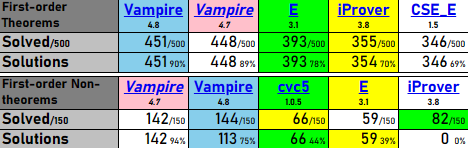
\includegraphics[width=0.5\textwidth]{CASC29.png}
		\caption{Results of CASC-29}
	\end{wrapfigure}

	Most modern provers are based on a form of ordered resolution~\cite{bachmair2001resolution}. The basic idea to determine the validity of a given formula is to transform the negated formula into a set of clauses, i.e. disjunctions of literals, and iteratively apply the rules from the calculus until the empty clause is derived, in which case the original formula is valid, or no more rules can be applied, i.e. the clause-set is saturated, in which case the original formula is valid. The calculus is refutationally complete, i.e. if the original formula is not valid the empty clause will be derived eventually. However, the search space is generally too large to be searched exhaustively, so provers employ a number of techniques to minimize the search space, e.g. different forms of redundancy~\cite{bachmair1994rewrite, hillenbrand2013search, gleiss2020subsumption}, and a whole suite of hyperparameters determining the search strategy, which are iteratively adjusted in portfolio modes~\cite{rawson2018dynamic}. More recently, machine learning techniques have been applied to direct search either by determining hyperparameters~\cite{bartek2020learning,bartek2023much}, or replacing the usual ordering-based search completely~\cite{jakubuuv2017enigma,kaliszyk2018reinforcement,crouse2021deep}. As such modern provers are enormously complex and evaluating new techniques is a challenging task~\cite{reger2014challenges}.


	\subsection{Intuitionistic Logic}

	Intuitionistic logic refers to a flavor of logic in which the existence of an object can only be established by explicit construction, as opposed to classical logic where existence can be shown implicitly, e.g. by assuming non-existence and deriving a contradiction.

	It essentially differentiates itself from classical logic by the fact that the law of excluded middle $A\vee\neg A$ and the double negation shift $\forall x\neg\neg P(x)\to\neg\neg\forall xP(x)$ are not valid.
	Besides philosophical considerations, most prominently advocated by Brouwer~\cite{brouwer1907over} and Bishop~\cite{bishop1967foundations}, there is a particular motivation for studying intuitionistic logic from the perspective of computer science in that proofs directly correspond to computer programs --- as expressed in the Curry--Howard correspondence~\cite{howard1980formulae}.
	
	This makes intuitionistic provers particularly interesting for program synthesis~\cite{alur2013syntax} as programs can be directly extracted from proofs. While classical proofs can also be equipped with program semantics~\cite{Parigot1,Control1} in general we at least lose realizability of existential quantifiers and disjunctions. While extracting witnesses from classical proofs is often possible~\cite{hozzova2023program}, in general a classical proof does not even guarantee the existence of a solution.
	
	Furthermore, most modern proof assistants such as Coq~\cite{bertot2013interactive} or Lean~\cite{de2015lean} are intuitionistic. Arguably one of the most effective automation tools for proof assistants is Sledgehammer~\cite{bohme2010sledgehammer} for Isabelle/HOL~\cite{nipkow2002isabelle}, which uses state-of-the-art classical first-order provers to find proofs for HOL problems. However, in proof assistants based on constructive type theory such as Coq or Lean, proofs generated in such a way can generally not be used. While such an approach has been attempted~\cite{czajka2018hammer}, it is limited in that it discards the generated proof and attempts to construct a new intuitionistic proof from the facts used in the classical proof. This is not always possible and even if it is the resulting proof can be much more complex than necessary. In contrast, an intuitionistic prover would be able to generate a proof that can be directly used in the proof assistant.

	\subsection{Automated theorem proving for intuitionistic logic}

	The interest in intuitionistic logic has lead to the development of a number of automated theorem proving systems and a collection of benchmark problems (see e.g. the ILTP library website~\cite{iltp}).
	The progress in automated reasoning for intuitionistic logic, however, has been slower than the  impressive advances in solvers for classic logics --- evidenced, e.g., by the CASC~\cite{casc} and SAT~\cite{satc} competitions.
	This difference can partially be explained by fundamental differences between the logics.
	First, determining intuitionistic validity is computationally harder, e.g., in the propositional case intuitionistic validity is \verb+PSPACE+-complete~\cite{statman1979intuitionistic}, whereas classical validity is \verb+coNP+-complete~\cite{cook1971complexity}.
	A further advantage of classical logic is the existence of calculi that are particularly suited for automation, such as ordered resolution~\cite{bachmair2001resolution}, which rely on the existence of convenient normal forms such as CNF, and the duality between validity and satisfiability (i.e., in order to show the validity of a formula it suffices to show the unsatisfiability of the negated formula, which is insufficient in intuitionistic logic).
	The first dedicated intuitionistic theorem provers~\cite{mclaughlin2009efficient,tammet1996resolution} used the naïve inverse method, i.e., a direct search for a cut-free proof by applying the rules from some proof calculus inversely, which generally leads to a very complex search.
	More recently, connection-based methods have been applied to various non-classical logics~\cite{otten2005clausal,otten2021nanocop}, including intuitionistic logic.
	There have also been some successful attempts to study intuitionistic validity via embedding into higher-order classical logic~\cite{LEO}.
	However, in comparison to classical provers, intuitionistic provers are much less mature and many modern techniques developed for classical provers have not been tested in an intuitionistic setting.

	\section{Research plan}

	\subsection{Research Questions and Methodology}

	\begin{question}
		Can a syntactic embedding of intuitionistic logic into classical logic be leveraged to efficiently decide intuitionistic validity using a classical prover? Can we retrieve intuitionistic proofs/counter-models from the corresponding classical proofs/counter-models?
	\end{question}

	\begin{method}
		Utilizing the Kripke semantics for intuitionistic logic we devise a dual embedding to the famous embedding of classical logic into intuitionistic logic by G\"odel~\cite{godel1933intuitionistischen}, i.e. we give a procedure that transforms each formula $\varphi$ into a formula $\varphi^C$ such that $\varphi$ is intuitionistically valid if and only if $\varphi^C$ is classically valid. We implement this embedding to work on a standard problem format like TPTP~\cite{tptp} and apply it to a benchmark set of intuitionistic problems, e.g. the ILTP benchmark set~\cite{iltp}. We then apply a state-of-the-art classical prover to the embedded problems and compare the performance to state-of-the-art intuitionistic provers. This question has been partially addressed in my master's thesis~\cite{thesis} and during the first year, resulting in a paper~\cite{pluska2023embedding}, more on this in the next section.
	\end{method}

	\vspace*{12pt}

	\begin{question}
		Can a more deep reflection of intuitionistic semantics in the proof calculus be used to leverage the power of modern classical provers for intuitionistic logic?
	\end{question}

	\begin{method}
		It is possible to embed intuitionistic semantics more deeply into a proof calculus than as a syntactic transformation of the formula. This has already been done in connection calculi~\cite{otten2005clausal}. We will modify the resolution calculus~\cite{bachmair2001resolution} to reflect intuitionistic semantics and implement this calculus in an existing prover, e.g. Vampire~\cite{kovacs2013first}. We will then compare the performance of this prover to state-of-the-art intuitionistic provers. Furthermore, we will experiment with other calculi and prover architectures.
	\end{method}

	\vspace*{12pt}

	\begin{question}
		Can we adapt modern techniques from classical provers to intuitionistic provers, in particular machine learning techniques?
	\end{question}

	\begin{method}
		State-of-the-art intuitionistic prover such as leanCoP~\cite{otten2008leancop} and nanoCoP~\cite{otten2021nanocop} are generally much simpler than state-of-the-art classical provers such as Vampire~\cite{kovacs2013first}, iProver~\cite{korovin2008iprover} or E~\cite{schulz2002brainiac}. On the one hand modern classical provers augment their calculus to utilize different forms of redundancy to minimize the search space~\cite{bachmair1994rewrite, hillenbrand2013search, gleiss2020subsumption} and on the other hand they utilize powerful portfolio modes~\cite{rawson2018dynamic} in order to optimize their large suites of hyperparameters. More recently, machine learning techniques have been applied to direct search either by determining hyperparameters~\cite{bartek2020learning,bartek2023much} or replacing the usual ordering-based search~\cite{jakubuuv2017enigma,kaliszyk2018reinforcement,crouse2021deep}. We will handpick a subset of these techniques that are particularly suited for intuitionistic logic and implement them in a state-of-the-art intuitionistic prover, e.g. nanoCoP~\cite{otten2021nanocop}. We will then compare the performance of this prover to state-of-the-art intuitionistic provers. In particular in case of machine learning techniques we expect benefits in terms of explainability and interpretability due to the lean underlying prover.
	\end{method}

	\vspace*{12pt}

	\begin{question}
		Can we use our findings to attain a new record on the ILTP benchmark~\cite{iltp}?
	\end{question}

	\begin{method}
		Applying the techniques developed in the previous questions we will work on a state-of-the-art intuitionistic prover either by extending an existing one, e.g. nanoCoP~\cite{otten2021nanocop}, equipping a classical solver with intuitionistic techniques, e.g. Vampire~\cite{kovacs2013first}, or developing a new one from scratch. We will then compare the performance of this prover to state-of-the-art intuitionistic provers.
	\end{method}

	\vspace*{12pt}

	\begin{question}
		Can we replace classical provers in settings where intuitionistic provers would be more suitable?
	\end{question}

	\begin{method}
		Sometimes it is desirable to obtain an intuitionistic proof for a problem rather than a classical one, e.g. in the context of proof assistants based on constructive type theory such as Lean~\cite{de2015lean} or Coq~\cite{bertot2013interactive} or in program synthesis~\cite{alur2013syntax}. There have been attempts to use classical provers in these contexts~\cite{czajka2018hammer,hozzova2023program}. However, these approaches are limited in that they cannot generally utilize the generated proof and a successful proof does not even guarantee the existence of a solution. We will investigate whether we can replace classical provers in these settings with intuitionistic provers. 
	\end{method}

	\vspace*{12pt}

	\begin{question}
		Can we efficiently find counter-models to intuitionistic validity?
	\end{question}

	\begin{method}
		Effectively finding counter-models in first-order logic is a long-standing challenge in automated reasoning~\cite{caferra1992method}. In resolution-based provers a counter-model can be constructed when the clause set reaches saturation~\cite{peltier2003model}. However, generally the clause set does not reach saturation and instead of finding a counter-model the prover will time out. In intuitionistic logic there are additional statements which have a counter-model, so the problem of finding one is of special interest. By reflecting the intuitionistic semantics deeply in the calculus~\cite{otten2005clausal} we can already find counter-models which we could not with a syntactic embedding~\cite{pluska2023embedding}, for example to the double negation shift
		\[\forall x\neg\neg P(x)\to\neg\neg\forall xP(x).\]
		We will examine what can be done to find counter-models to intuitionistic validity and work on representation and visualization of such counter-models. Furthermore, we will investigate if we can transfer some of our findings back to classical solvers, as such this question is more open-ended than the others.
	\end{method}

	\subsection{Current state of research}

	\begin{wrapfigure}[5]{r}{0.43\textwidth}
		\vspace*{-1cm}
		\begin{tabular}{l|c|c}
			Embedding&571&21.4\%\\
			ileanCoP 1.2&875&32.8\%\\
			nanoCoP-i 2.0&858&32.1\%\\\hline
			Total&2669&100\%
		\end{tabular}
		\caption{Solved problems.}
		\label{fig:a}
	\end{wrapfigure}

	Q1 has been addressed during my master's thesis and the findings have been refined and during the first year of my dissertation, resulting in a paper~\cite{pluska2023embedding}. While a purely syntactic embedding utilizing state-of-the-art classical provers was able to compete with state-of-the-art intuitionistic provers on certain subclasses of benchmarks it came short on the general benchmark set as can be seen in Figure~\ref{fig:a}. However, the embedding was able to solve a number of problems that the intuitionistic provers could not solve. After publication, beyond an external embedding tool~\cite{embedding} we have implemented a preprocessing option in the Vampire theorem prover~\cite{vampireintuitionistic} performing the syntactic embedding. Finally, we have also determined how to retrieve intuitionistic proofs/counter-models from their classical counter-parts in this setting. As we don't see significant potential for improvement from a purely syntactical approach Q1 is considered answered. We observed that a significant portion of problems which the embedding could not solve but the intuitionistic provers could solve were not intuitionistically valid.
	
	This is a promising sign for Q2 as a more deep embedding into the calculus would be able to determine counter-satisfiability in such cases. We have already begun equipping Vampire~\cite{kovacs2013first} with intuitionistic techniques, in particular we need to store for each literal a string that represents a set of worlds in a potential Kripke countermodel and to modify unification to respect this information. As Vampire is quite complex, this comes with a number of engineering challenges. Furthermore, we must ensure that our modifications play well with the existing techniques in Vampire, e.g. different forms of redundancy~\cite{gleiss2020subsumption}, so that the calculus remains at least sound and ideally refutationally complete.

	Addressing Q3 also requires some groundwork. In order to experiment with different classical techniques in an intuitionistic prover we need to establish a framework which allows fast iteration and testing, in particular of machine learning techniques. As such we have decided on a Python-based frontend. The connection calculi have been originally implemented in PROLOG and understanding how to replicate their exact functionality is a challenge. Furthermore, most techniques that have been examined in classical provers based on ordered resolutions will need to be adjusted to our setting.

	We have not begun to address Q4-6 yet as outlined in the timeline below.

	\subsection{Lectures and Teaching}

	I plan to attend the following lectures:

	\begin{itemize}
		\item\textbf{184.766 Introduction to Logical Methods in Computer Science}\\Apart from a refresher, this lecture will also be an opportunity to learn about adjacent fields and connect with other researchers.
		\item \textbf{Guest Professor’s Course}\\Based on availability a relevant lecture conducted by a guest professor will be attended.
		\item \textbf{195.098 Research and Career Planning for Doctoral Students}\\This lecture will help me to understand the requirements of a successful career and to plan my dissertation and future accordingly.
		\item \textbf{195.080 Philosophy of Science}\\This lecture will allow me to reflect on my research from a philosophical perspective and place it in a broader context.
		\item \textbf{194.101 Machine Learning Algorithms and Applications}\\Given my limited background in applied machine learning, this project will allow me to better understand and classify some modern techniques used in classical provers as well as allow me to implement some of them myself.
		\item \textbf{194.077 Applied Deep Learning}\\As above, this lecture will allow me to better understand deep learning approaches to automated reasoning.
	\end{itemize}
	During the first year I have been involved in the teaching of the following courses:
	\begin{itemize}
		\item \textbf{185.291 Formal Methods in Computer Science}
		\item \textbf{185.A93 Formal Methods in Computer Science}
	\end{itemize}
	I have coordinated the design and grading of exams and exercises for Block 4 of the lecture and its exercise part. Furthermore, I have conducted two tutorials and answered students' questions. I plan to continue this involvement.

	\subsection{Timeline}

	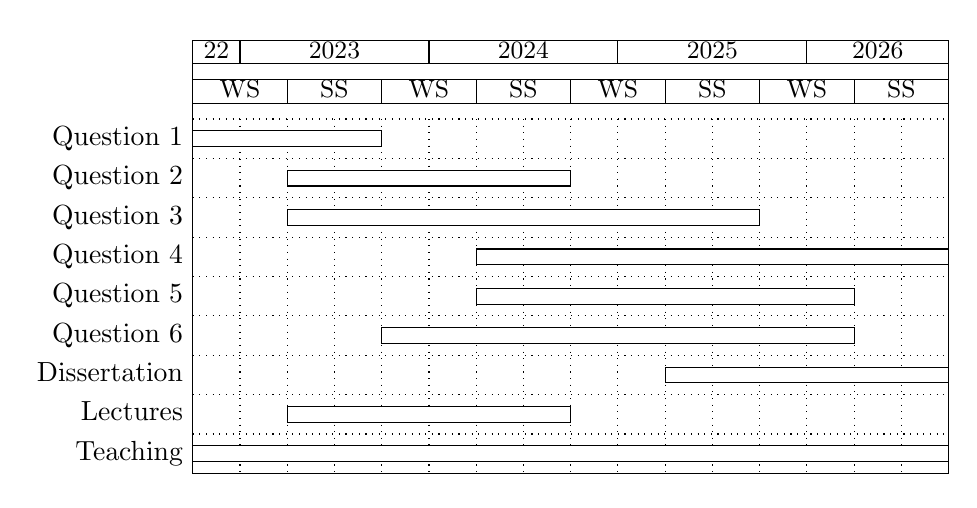
\begin{tikzpicture}
		\begin{ganttchart}[vgrid, hgrid, x unit=.6cm, y unit title=0.5cm, y unit chart=0.5cm]{1}{16}
			\gantttitle{22}{1}
			\gantttitle{2023}{4}
			\gantttitle{2024}{4}
			\gantttitle{2025}{4}
			\gantttitle{2026}{3}\\
			\gantttitle{WS}{2}
			\gantttitle{SS}{2}
			\gantttitle{WS}{2}
			\gantttitle{SS}{2}
			\gantttitle{WS}{2}
			\gantttitle{SS}{2}
			\gantttitle{WS}{2}
			\gantttitle{SS}{2}\\
			\ganttbar{Question 1}{1}{4}\\
			\ganttbar{Question 2}{3}{8}\\
			\ganttbar{Question 3}{3}{12}\\
			\ganttbar{Question 4}{7}{16}\\
			\ganttbar{Question 5}{7}{14}\\
			\ganttbar{Question 6}{5}{14}\\
			\ganttbar{Dissertation}{11}{16}\\
			\ganttbar{Lectures}{3}{8}\\
			\ganttbar{Teaching}{1}{16}
		\end{ganttchart}
	\end{tikzpicture}

	As explained above, Q1 can be considered answered. Q2 and Q3 are currently being addressed. Q2 is mostly an implementation effort, for which the biggest challenge is understanding all the details of the Vampire system, we expect to have a working prototype at the latest by the end of the second year. Q3 is a more open-ended question and will require experimentation. As it is difficult to foresee which approaches will be successful it is difficult to give a definite timeline, and we expect to keep improving upon our results throughout the dissertation.
	Q4 and Q5 build on the results of Q2 and Q3 and will be addressed in the second half of the dissertation, we have conducted some preliminary work to utilize intutionstic provers in proof assistants, but this can only be evaluated properly once Q2 and Q3 are answered. Finally, Q6 can be approached in different ways and addressed in parallel to the other questions. It will be a continuous effort, but the other questions will take priority.

	The dissertation will be written in the last 18 months of the project. By then we expect to have at least partial answers to Q1-5 and a good understanding of the remaining open questions, which should be sufficient to begin writing.

	I plan to attend the required lectures within the first 2 years. I will continue to be involved in teaching throughout the project.

	\subsection{Conferences and Workshops}

	I have attended LPAR-24 at which my paper~\cite{pluska2023embedding} was accepted. I plan to attend further venues at which I can present my work. Furthermore, I plan to attend workshops and conferences relevant to my research.

	\bibliographystyle{acm}
	\bibliography{bibliography}
	
\end{document}